\documentclass[a4paper,12pt,oneside]{report}
\usepackage{graphicx}
\usepackage{color}
\usepackage{url}
\usepackage{subfigure}
\usepackage[utf8]{inputenc}
\usepackage[T1]{fontenc}
\usepackage{tgpagella}
\usepackage{xstring}
\usepackage{wrapfig}
\usepackage{appendix}
\usepackage{nomencl}
\usepackage{algorithm}
\usepackage{algorithmic}
\usepackage{multicol}
\usepackage[pdfborder=0 0 0]{hyperref}

\newcommand{\myscale}{0.74}
\newcommand{\vect}[1]{\boldsymbol{#1}}
\newcommand{\code}[1]{\texttt{\StrSubstitute{#1}{.}{.\.}}}
\def\.{\discretionary{}{}{}}
\newcommand{\heu}[1]{\texttt{\textit{#1}}}
\newcommand{\jmodule}[1]{\texttt{\textit{#1}}}
\linespread{1.5}

\renewcommand{\algorithmicrequire}{\textbf{Input:}}
\renewcommand{\algorithmicensure}{\textbf{Output:}}
\renewcommand{\algorithmicforall}{\textbf{for each}}
\renewcommand{\algorithmiccomment}[1]{\textit{// #1}}

\setlength{\hoffset}{-1in} %left margin will be 0, as hoffset is by default 1inch
\setlength{\voffset}{-1in} %analogous voffset
\setlength{\oddsidemargin}{4cm}
\setlength{\evensidemargin}{4cm}
\setlength{\topmargin}{25mm}
\setlength{\footskip}{1cm}
\setlength{\headheight}{0cm}
\setlength{\headsep}{0cm}
\setlength{\marginparwidth}{0cm}
\setlength{\marginparpush}{0cm}
\setlength{\textheight}{23.7cm}
\setlength{\textwidth}{14.5cm}
\let\openright=\clearpage

\def\mfauthor{Matej Vitásek}
\def\mfadvisor{RNDr. Irena Mlýnková Ph.D.}
\def\mfplacedate{Praha, 2011}

% Tato makra přesvědčují mírně ošklivým trikem LaTeX, aby hlavičky kapitol
% sázel příčetněji a nevynechával nad nimi spoustu místa. Směle ignorujte.
\makeatletter
\def\@makechapterhead#1{
  {\parindent \z@ \raggedright \normalfont
   \Huge\bfseries \thechapter. #1
   \par\nobreak
   \vskip 20\p@
}}
\def\@makeschapterhead#1{
  {\parindent \z@ \raggedright \normalfont
   \Huge\bfseries #1
   \par\nobreak
   \vskip 20\p@
}}
\makeatother

\def\chapwithtoc#1{
\chapter*{#1}
\addcontentsline{toc}{chapter}{#1}
}

\renewcommand{\nomname}{List of Abbreviations}
\makenomenclature

\begin{document}

\lefthyphenmin=2
\righthyphenmin=2

%%% Titulní strana práce ======================================================
\pagestyle{empty}
\begin{center}

\large

Charles University in Prague

\medskip

Faculty of Mathematics and Physics

\vfill

{\bf\Large MASTER THESIS}

\vfill

\centerline{\mbox{
\includegraphics[width=60mm]{logo.eps}}}

\vfill
\vspace{5mm}

{\LARGE \mfauthor}

\vspace{15mm}

% exactly as assigned
{\LARGE\bfseries Inference of XML Integrity Constraints}

\vfill

% Název katedry nebo ústavu, kde byla práce oficiálně zadána
% (dle Organizační struktury MFF UK)
Department of Software Engineering

\vfill

\begin{tabular}{rl}

Supervisor of the master thesis: & 	\mfadvisor \\
\noalign{\vspace{2mm}}
Study programme: & Informatika \\
\noalign{\vspace{2mm}}
Specialization: & ISS \\
\end{tabular}

\vfill

% Zde doplňte rok
\mfplacedate 

\end{center}



\newpage % ============================================================
%%% Následuje vevázaný list -- kopie podepsaného "Zadání diplomové práce".
%%% Toto zadání NENÍ součástí elektronické verze práce, nescanovat.
\openright

\noindent
[Sample: Here you may thank whoever you wish (the supervisor of the thesis, the consultant,
the person who lent the software, literature, etc.)]

TODO thank jInfer team, Mlynkova, anyone helping create this, colleagues at work...


\newpage % ============================================================
%%% Strana s čestným prohlášením k diplomové práci
\vglue 0pt plus 1fill
\noindent
I declare that I carried out this master thesis independently, and only with the cited
sources, literature and other professional sources.

\medskip\noindent
I understand that my work relates to the rights and obligations under the Act No.
121/2000 Coll., the Copyright Act, as amended, in particular the fact that the Charles
University in Prague has the right to conclude a license agreement on the use of this
work as a school work pursuant to Section 60 paragraph 1 of the Copyright Act.

\vspace{10mm}

\hbox{\hbox to 0.5\hsize{%
In ........ date ............
\hss}\hbox to 0.5\hsize{%
signature
\hss}}

\vspace{20mm}



\newpage % ============================================================
%%% Povinná informační strana diplomové práce
\vbox to 0.5\vsize{
\setlength\parindent{0mm}
\setlength\parskip{5mm}

Název práce: Odvozování integritních omezení v XML % TODO how to translate this correctly?

Autor: \mfauthor

Katedra:  Katedra softwarového inženýrství

Vedoucí diplomové práce: \mfadvisor{}, Katedra softwarového inženýrství

Abstrakt: [abstract of 80-200 words in Czech, but not a copy of the assignment of the
master thesis]

Klíčová slova:  XML, ID atributy, odvozování

\vss}\nobreak\vbox to 0.49\vsize{
\setlength\parindent{0mm}
\setlength\parskip{5mm}

Title:  Inference of XML Integrity Constraints

Author: \mfauthor

Department: Department of Software Engineering

Supervisor: \mfadvisor{}, Department of Software Engineering

Abstract:  [abstract of 80-200 words in English, but not a copy of the assignment of
the master thesis]

Keywords: XML, ID attributes, inference

\vss}

\newpage

%%% Strana s automaticky generovaným obsahem diplomové práce. U matematických
%%% prací je přípustné, aby seznam tabulek a zkratek, existují-li, byl umístěn
%%% na začátku práce, místo na jejím konci.

\openright
\pagestyle{plain}
\setcounter{page}{1}
\tableofcontents

% =============== TEXT ================
\newpage

% TODO what style of quotation marks to use? 
% TODO how to format text? is textit / texttt / ... OK?

\chapwithtoc{Preface}

Along with technologies like JSON, SQL/noSQL databases and bla, XML is one of the leading formats for storing structured data. However, even though languages such as DTD and XML Schema to describe XML structure already exist since a long time, most of the documents use outdated or no schema at all (link Vosta's Even ant can create...). To tackle this problem one may employ reverse-engineering techniques to infer the schema from existing documents, such as those described in A, B, C, jInfer. But the schema is not the only constraint that can be imposed on an XML document: the concept of \textit{keys} and \textit{foreign keys}, well known from the relational database world, applies here as well. One could go even further and try to find even more sophisticated relations in the data, such as \textit{functional dependencies} (link Sviro).

This work will be building upon the achievements of jInfer schema inference framework (TODO link Anti's improvements in schema inference), expanding its possibilities in the field of search for \textit{key-} and \textit{foreign key-}like structures in existing XML documents.

TODO Integrity constraints can be keys (with ID attributes as a "sub-group"), FKs, functional dependencies (quote Sviro), etc.
We will focus on the first kind - ID and IDREF attributes.

TODO argument: test data with DTD (and thus possibly ID/IDREF) is more common, we can have better test sets.

\section{Structure of the thesis}

The thesis will be structured as follows. 

First, we will introduce a few notions required throughout the work, such as XML tree, ID attributes, ID sets and keys for XML. 

Secondly, we will review approaches to ID attribute and XML keys search from previous articles on this topic. 

This will lead us to the NP-complete problem of maximal independent set (IS)\nomenclature{IS}{Independent Set}, where we will inspect approaches for solving it.

We will discuss a closely related Mixed Integer Problem (MIP)\nomenclature{MIP}{Mixed Integer Problem} and prove their "equality".

Afterwards, we will show how to use an external MIP solver and various heuristics to tackle this problem.

An extension to jInfer for finding ID attributes using MIP solver and a combination of heuristics will be presented and experimentally evaluated in the closing chapters.

\chapter{Definitions}

\begin{itemize}
	\item XML tree - from FIDAX or wherever
	\item Element, Attribute
	\item ID, IDREF, IDREFS attribute according to specification
	\item XSD keys (compare them to ID attributes)
	\item Key according to Keys for XML \cite{keX}
	\item Attribute mapping \nomenclature{AM}{Attribute Mapping}
	\item ID set
  \item Weight: support, coverage
\end{itemize}

\chapter{Research}

According to the article \cite{fidax}, ...

TODO talk about FIDAX
To the best of our knowledge, there are no other articles dealing with this problem. 

TODO talk about Fajt - but that's different, that's keys
TODO add citation for Fajt

\section{Independent Set}

TODO define IS + MIS rigorously

TODO other approaches to max IS

\chapter{MIP Approach}

TODO rigorously define MIP - optimization problem, some of the variables integral

TODO FIDAX is cool, but their heuristic might not be the best. It is a IS problem, let's try a multi-purpose solver. Use GLPK. \nomenclature{GLPK}{GNU Linear Programming Kit}

\section{Finding ID sets with GLPK}

TODO how GLPK works (branch \& bound), how to construct a problem, how output looks, how to interpret it, limit time-> limit quality, ...
 
 -> wow, GLPK works. However, it takes too long to get to optimum (link experiments), so let's try other heuristics.
 
\section{Heuristics}

TODO what is heuristics (link wise books), what is metaheuristics (we will be using them)

TODO mention things like Taboo search and Genetic Algorithms (we can emulate them with Crossover/Mutation) (we won't be using them)

TODO we will be working with heuristics striving to do the following: input is a list of AMs, they have their weight, we try to find a non-conflicting subset which maximizes the weight

TODO we will be using a pool - what is a pool

\begin{figure}
  \caption{Metaheuristic schema}
  \label{image-metaheuristic}
  \centering
    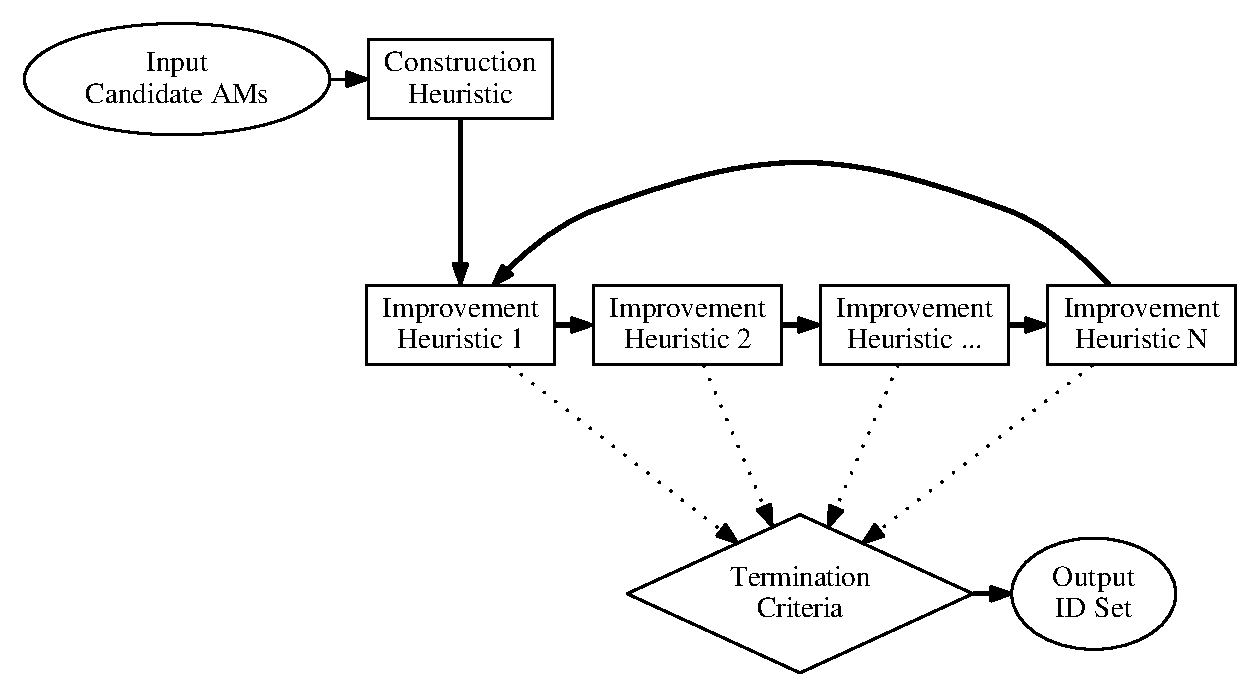
\includegraphics[width=\textwidth]{images/metaheuristic.eps}
\end{figure}

\subsection{Constructions Heuristics}
% TODO can I format things in nomenclature?
\nomenclature{CH}{Construction Heuristic} %TODO decide on how to format CH/IH 

TODO construction heuristics are heus that provide us with at least some solution.

\subsubsection{FIDAX}

TODO this is a heuristic too! We can start with it!

The pseudocode is listed (cited from \cite{fidax} with trivial modifications without changing the logic) in \ref{ch-fidax}.

\begin{algorithm}
\caption{FIDAX CH}
\label{ch-fidax}
\begin{algorithmic}
\REQUIRE $C$ list of candidate AMs
\STATE $C' \gets C$ sorted by decreasing size
\STATE Compute the weight $w(m)$ of each $m$ in $C$
\FORALL{$t$ in $\Sigma^E$}
  \STATE Let $m$ be a \textbf{highest-weight} mapping of type $t$ in $C'$
  \STATE Remove from $C'$ all mappings of type $t$ except $m$
\ENDFOR
\FORALL{$m$ in $C'$}
  \STATE $S \gets$ all mappings in $C$ whose images intersect $\iota(m)$
  \IF{$w(m) > \sum_{p \in S} w(p)$}
    \STATE remove all $p \in S$ from $C'$
  \ELSE
    \STATE remove $m$ from $C'$
  \ENDIF
\ENDFOR
\RETURN $C'$
\end{algorithmic}
\end{algorithm}

\subsubsection{Random}

TODO this is trivial, but works - link experiments where it bashes FIDAX

See listing \ref{ch-random}.

\begin{algorithm}
\caption{Random CH}
\label{ch-random}
\begin{algorithmic}
\REQUIRE $N$ required size of pool
\REQUIRE $C$ list of candidate AMs
\ENSURE pool of $N$ feasible solutions
\STATE $r \gets $ empty pool
\FOR{$i = 1 \to N$} 
  \STATE \COMMENT{create 1 solution}
  \STATE $s \gets $ empty solution
  \WHILE{$s$ is a feasible ID set}
    \STATE $a \gets $ pick at random from $C \backslash S$
    \STATE $s \gets s \cup a$
  \ENDWHILE
  \STATE $r \gets r \cup s$
\ENDFOR
\RETURN $r$
\end{algorithmic}
\end{algorithm}

\subsubsection{Fuzzy}

TODO kind of trivial

See listing \ref{ch-fuzzy}.

\begin{algorithm}
\caption{Fuzzy CH}
\label{ch-fuzzy}
\begin{algorithmic}
\REQUIRE $N$ required size of pool
\REQUIRE $C$ list of candidate AMs
\ENSURE pool of $N$ feasible solutions
\STATE $r \gets $ empty pool
\FOR{$i = 1 \to N$} 
  \STATE \COMMENT{create 1 solution}
  \STATE $s \gets $ empty solution
  \STATE $C' \gets C$

  \WHILE{$C' $ not empty}
    \STATE $a \gets $ pick at weighted random from $C'$
    \IF{$s \cup a$ is a feasible ID set}
      \STATE $s \gets s \cup a$
      \STATE $C' \gets C' \backslash a$
    \ENDIF
    \FORALL{$c \in C'$}
      \IF{$s \cup c $ is \textbf{not} a feasible ID set}
        \STATE \COMMENT {if $c$ cannot be possibly added anymore}
        \STATE $C' \gets C' \backslash c$
      \ENDIF
    \ENDFOR
  \ENDWHILE

  \STATE $r \gets r + s$
\ENDFOR
\RETURN $r$
\end{algorithmic}
\end{algorithm}

\subsubsection{Incremental}

TODO trivial, hungry, always 1 solution

See listing \ref{ch-incremental}.

\begin{algorithm}
\caption{Incremental CH}
\label{ch-incremental}
\begin{algorithmic}
\REQUIRE $C$ list of candidate AMs
\ENSURE a feasible solution
\STATE $C' \gets $ sort $C$ by decreasing weight
\STATE $s \gets $ empty solution
\FORALL{$c \in C'$}
  \IF{$s \cup c$ is a feasible ID set}
    \STATE $s \gets s + c$
  \ENDIF
\ENDFOR
\RETURN $s$
\end{algorithmic}
\end{algorithm}

\subsubsection{Removal}

TODO trivial, "hungry", always 1 solution

See listing \ref{ch-removal}.

\begin{algorithm}
\caption{Removal CH}
\label{ch-removal}
\begin{algorithmic}
\REQUIRE $C$ list of candidate AMs
\ENSURE a feasible solution
\STATE $C' \gets $ sort $C$ by increasing weight
\STATE $s \gets C'$
\FORALL{$c \in s$}
  \IF{$s$ is a feasible ID set}
    \RETURN $s$
  \ENDIF
  \STATE $s \gets s \backslash c$
\ENDFOR
\end{algorithmic}
\end{algorithm}

\subsubsection{Truncated Branch \& Bound}

TODO if we limit GLPK's runtime, we get this 

\subsection{Improvement Heuristics}

\nomenclature{IH}{Improvement Heuristic}

TODO what they are, that they need a pool sometimes, their input and output is a pool, ...

TODO mention intensification, diversification

\subsubsection{Identity}

This ultimately trivial improvement heuristics does nothing. It simply returns the feasible pool unchanged. For the sake of completeness, see its listing \ref{ih-identity}.

\begin{algorithm}
\caption{Identity IH}
\label{ih-identity}
\begin{algorithmic}
\REQUIRE $FP$ pool of feasible solutions
\ENSURE the same pool of feasible solutions
\RETURN $FP$
\end{algorithmic}
\end{algorithm}

\subsubsection{Remove Worst}

TODO trivial

See listing \ref{ih-removeworst}.

\begin{algorithm}
\caption{Remove Worst IH}
\label{ih-removeworst}
\begin{algorithmic}
\REQUIRE $FP$ pool of feasible solutions
\ENSURE pool of feasible solutions
\STATE $s_{min} \gets $ solution with the lowest weight $\in FP$
\RETURN $FP \backslash s_{min}$
\end{algorithmic}
\end{algorithm}

\subsubsection{Random Remove}

TODO trivial, perturbation

See listing \ref{ih-randomremove}.

\begin{algorithm}
\caption{Random Remove IH}
\label{ih-randomremove}
\begin{algorithmic}
\REQUIRE $FP$ pool of feasible solutions
\REQUIRE $k \in (0,1)$ ratio of AMs to remove from each $s \in FP$
\ENSURE pool of feasible solutions
\FORALL{$s \in FP$}
  \STATE $K \gets k * |s|$
  \STATE remove $K$ random AMs from $s$
\ENDFOR
\RETURN $FP$
\end{algorithmic}
\end{algorithm}

\subsubsection{Hungry}

This simple improvement heuristic assumes that the solutions in the pool are not ``complete", i.e. there are AMs that could be added to them without violating the ID set condition.

\heu{Hungry} tries to improve each solution in the feasible pool in the following way. It orders all candidate AMs not present in the solution by decreasing weight. Afterwards, it iteratively tries to extend the solution with these AMs, taking care not to violate the ID set condition. The resulting solution (whether any AMs were added or not) is then returned to the pool. Listing \ref{ih-hungry} captures this process.

\begin{algorithm}
\caption{Hungry IH}
\label{ih-hungry}
\begin{algorithmic}
\REQUIRE $FP$ pool of feasible solutions
\REQUIRE $C$ list of candidate AMs
\ENSURE pool of feasible solutions
\FORALL{$s \in FP$}
  \STATE \COMMENT {improve a single solution}
  \STATE $C' \gets C \backslash s$
  \STATE $C' \gets C'$ sorted by decreasing weight
  \FORALL{$c \in C'$}
    \IF{$s \cup c$ is a feasible ID set}
      \STATE $s \gets s \cup c$
    \ENDIF
  \ENDFOR
\ENDFOR
\RETURN $FP$
\end{algorithmic}
\end{algorithm}

\subsubsection{Mutation}

TODO explain how this translates to GLPK input

See listing \ref{ih-mutation}.

\begin{algorithm}
\caption{Mutation IH}
\label{ih-mutation}
\begin{algorithmic}
\REQUIRE $FP$ pool of feasible solutions
\REQUIRE $k$ ratio of AMs to fix
\ENSURE pool of feasible solutions
\STATE $incumbent \gets $ best solution in $FP$ \COMMENT {best = highest weight}
\STATE $K \gets k * |incumbent|$
\STATE fix $K$ random AMs from $incumbent$ in GLPK problem formulation
\STATE $improved \gets $ run GLPK
\RETURN $FP \cup improved$
\end{algorithmic}
\end{algorithm}

\subsubsection{Crossover}

TODO explain how this translates to GLPK input

See listing \ref{ih-crossover}.

\begin{algorithm}
\caption{Crossover IH}
\label{ih-crossover}
\begin{algorithmic}
\REQUIRE $FP$ pool of feasible solutions
\REQUIRE $k$ ratio of solutions to look for commonalities in
\ENSURE pool of feasible solutions
\STATE $K \gets k * |FP|$
\STATE $FP' \gets K$ random solutions $\in FP$
\STATE $am \gets$ AMs found in all solutions $\in FP'$
\STATE fix $am$ in GLPK problem formulation
\STATE $improved \gets $ run GLPK
\RETURN $FP \cup improved$
\end{algorithmic}
\end{algorithm}

\subsubsection{Local Branching}

TODO explain how this translates to GLPK input

See listing \ref{ih-localbranching}.

\begin{algorithm}
\caption{Local Branching IH}
\label{ih-localbranching}
\begin{algorithmic}
\REQUIRE $FP$ pool of feasible solutions
\REQUIRE $k$ ratio of total AM count to bound the Hamming distance to
\ENSURE pool of feasible solutions
\STATE $K \gets k * |$total AM count$|$
\STATE $incumbent \gets $ best solution in $FP$ \COMMENT {best = highest weight}
\STATE add max Hamming distance requirement to GLPK problem formulation
\STATE $improved \gets $ run GLPK
\RETURN $FP \cup improved$
\end{algorithmic}
\end{algorithm}

\section{IDREF}

TODO describe the (rather trivial) algorithm of finding IDREF attributes once we have the ID set

\chapter{Experiments}

TODO describe all the inputs (take it from the mindmap), describe how the output looks (sample trace - link to appendix)

\section{Experimental Data}

TODO types of data:
\begin{itemize}
	\item Realistic 
	\item Realistic with artificial attributes
	\item Artificial
\end{itemize}

TODO for all types, show GraphViz pictures.

\subsection{Realistic data}

TODO talk about all that are used - mention the dataset name, some characteristics (excel sheet)

\subsection{Realistic data with artificial attributes}

TODO we have taken some of the text data and converted it to attributes like this, A B C

\subsection{Artificial data}

TODO these are random graphs.
TODO talk about how they are created, about their structure.
TODO talk about some "density".

\section{Experimental Setup}

TODO we will be using jInfer and its module AttributeStats see \ref{jInfer} and \ref{attrstats}.
TODO describe how to create a model, describe how we get IGG, link BasicIGG

\section{Experimental Results}

TODO following experiments + more

\begin{itemize}
	\item For each input file: how long does model creation take?
	\item How long does it take to communicate with GLPK? Creating the input/parsing the output.
	\item Which construction heuristic is the best - limit GLPK to like 1 second
	\item With the best construction heuristic, which IH is the best? Note that this needn't be the best combination!
	\item With the best IH from the previous step, how about using Random as CH?
	\item GLPK: Input -> How long the search for optimum lasts - this shows we cannot rely on GLPK alone! it just takes too long.
	\item GLPK: Time limit -> Quality
	\item Structure of the data -> Which algorithms perform the best
	\item Alpha, Beta -> Quality
	\item Alpha, Beta -> How does the solution work?
	\item Which GLPK -> How does (time->quality) look, how does (input->time) look
	\item Do I beat FIDAX with Random?
	\item Does Fuzzy beat Random? (Seems that Random is better and even has smaller variance)
\end{itemize}

\section{The "Best" Algorithm}

TODO we have asked a lot of questions and got the answers, now is the time to summarize, to find some "wisdom".

First of all: if we have the time, it is best to just let the GLPK run. 
We will find the optimum in this way. 
And for many purposes, this is just fine - we need to infer something about the schema, we do it only once, so it doesn't matter that much how long it takes.

Second: if we don't have enough time, we should do XYZ but it might depend on the characteristics of the data.
For realistic (looks like THIS in graph representation) it is best to do A B C.
Whereas, for artificial data (having IJK as their representation) it is best to just do 1 2 3.

\chapter{Future work}

TODO extension to more documents, IDREFs, ...  

\chapwithtoc{Conclusion}

TODO conclusion: From all integrity constraints in XML we chose the ID attributes and decided to improve the search for them. We discussed the approach chosen in FIDAX. Based on this article we introduced the MIP approach and demonstrated how to find the optimal (w.r.t. weight) ID set.

However, this approach takes too long for some inputs, so we introduced a whole spectrum of construction as well as improvement heuristics. By combining these algorithms and tuning their parameters we were able to find very good solutions while maintaining low running times.

%%% Seznam použité literatury
\newpage
\nocite{*}
\bibliographystyle{alpha}
\bibliography{literature}

\listoffigures
\addcontentsline{toc}{chapter}{List of Figures}

\listofalgorithms
\addcontentsline{toc}{chapter}{List of Algorithms}

%%% Tabulky v diplomové práci, existují-li.
%\chapwithtoc{List of Tables}
\listoftables
\addcontentsline{toc}{chapter}{List of Tables}

%%% Použité zkratky v diplomové práci, existují-li, včetně jejich vysvětlení.

\printnomenclature[2cm]
\addcontentsline{toc}{chapter}{List of Abbreviations}

%%% Přílohy k diplomové práci, existují-li (různé dodatky jako výpisy programů,
%%% diagramy apod.). Každá příloha musí být alespoň jednou odkazována z vlastního
%%% textu práce. Přílohy se číslují.

\appendix

\openright
\addcontentsline{toc}{chapter}{Appendices}

\chapter{jInfer}
\label{jInfer}

This appendix will try to describe shortly yet comprehensively \textbf{jInfer} - the Java framework for XML schema inference. Please see TODO link jInfer project web for complete information, documentation and download options.

jInfer was developed between 2009 and 2011 at Charles University in Prague as a Software Project by team consisting of Michal Klempa, Mario Mikula, Robert Smetana, Michal Svirec and Matej Vitasek. The main idea was to create a structure in which all aspects of XML schema inference can be easily implemented and evaluated. The goal was apparently achieved: the SW project was successfuly defended when jInfer was inferring DTD and XSD schemas based on XML documents, old DTD and XSD schemas and XPath queries. Since then, Michal Klempa has successfuly defended his own thesis improving on the grammar simplification process (see below), Michal Svirec has extended the framework with capabilities to detect and repair functional dependencies violation and defended his thesis as well. This thesis is the third based on this framework, and Mario Mikula's is on its way, too.

At heart of jInfer inference process is a modular system provided by NetBeans Platform allowing to define services (interfaces), implement them in any number of ways and then let the user choose which implementation to use. Most importantly, the whole process consists of 3 consecutive steps (see \ref{image-inference-process}), responsibility of 3 different services - interchangeable modules.

\begin{figure}
  \caption{Inference process in jInfer}
  \label{image-inference-process}
  \centering
    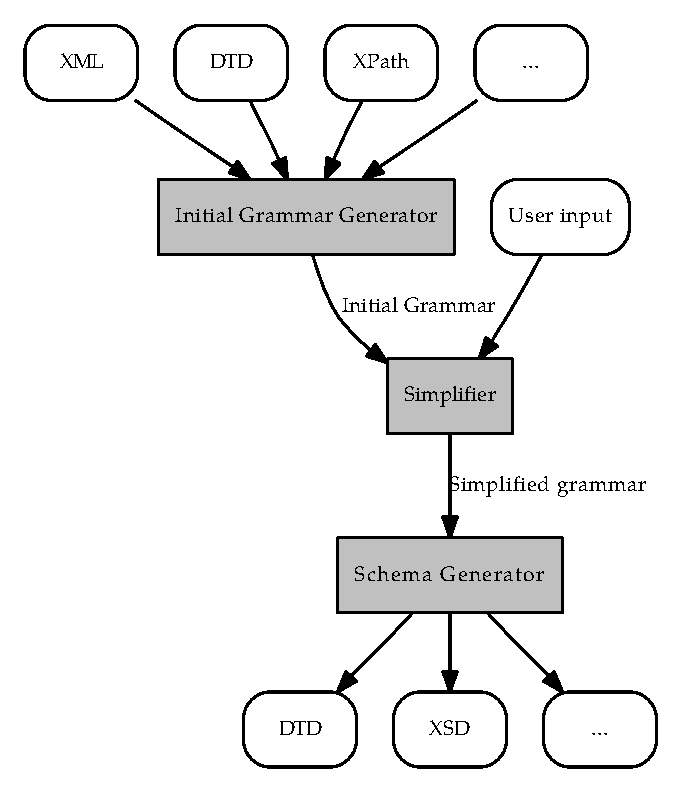
\includegraphics[width=0.5\textwidth]{images/inference-process.eps}
\end{figure}

The responsibility of the first module, the \jmodule{Initial Grammar Generator}, is to parse all input files (documents, schemas and queries) and create a so-called \textit{initial grammar} (IG, TODO nomenclature). This is the representation in which will the structure live until it is used to create the final product - the schema. As the name suggests, IG is a grammar - an \textit{extended context-free grammar}, to be more precise (TODO link CFGs). As such, its left hand side is an element, its right hand side is a regular expression representing its content model. (TODO picture?) IG is used to create the AM model used in this thesis, too. jInfer contains one such module, the \jmodule{BasicIGG}, which is described in detail in (TODO link BasicIGG documentation).

After leaving the \jmodule{Initial Grammar Generator}, the IG needs to be made more general, shortened, \textit{simplified}. This is the responsibility of an aptly named module, the \jmodule{Simplifier}. To get the full idea about how this can be done it would be probably best to read Michal Klempa's thesis (TODO link), which describes this in great detail. Whatever happens, there is simplified grammar on the exit of \jmodule{Simplifier}, ready to be processed by...

The last module, \jmodule{Schema Generator} takes the simplified grammar and creates the resulting schema from it. This process is not too interesting, but anyone wishing to find out all about it is invited to read the documentation to the two \jmodule{Schema Generator}s bundled with jInfer - the BasicDTD and BasicXSD modules.

TODO elaborate more, if too short:)

\chapter{IDSetSearch}
\label{iss}

TODO talk a bit about the structure of ISS module.

\chapter{Traces}
\label{traces}

Following is a trace logged from a sample experiment run. It shows all the relevant information related to this instance, any and every piece of information we might be interested in.

To save space, 2-column layout is used. Commentary on the particulars follows right after its end.

\begin{multicols}{2}
\begin{scriptsize}
\begin{verbatim}
CPU info
  Intel(R) Core(TM)2 Quad CPU Q9550 @ 2.83GHz
  Cores: 4
  Clock speed: 2983 MHz
Memory info
  Size: 8192 MB
OS info
  Name: Windows 7
  Version: 6.1
  Architecture: amd64
Java info
  Version: 1.6.0_26
  VM: Java HotSpot(TM) 64-Bit Server VM
GLPK info
  GLPSOL: GLPK LP/MIP Solver 4.34

Configuration:
File name: graph.xml (101599 b)
  Graph representation: 82 vertices, 1101 edges
alpha: 1.0, beta: 1.0

Results:
Start time: Thu Jan 01 01:22:17 CET 1970
Total time spent: 7754 ms
Final quality: 0.19951219512195123 (10 AMs)
Highest quality: 0.23463414634146343 (12 AMs)
Construction phase: 
  Algorithm: Random
    Time taken: 248 ms
    Time since start: 248 ms
    Pool size: 10
    Quality: 0.19975609756097568 (11 AMs)
Improvement phase: 
  pass #1: 
  Algorithm: RandomRemove, ratio = 0.2
    Time taken: 0 ms
    Time since start: 841 ms
    Pool size: 10
    Quality: 0.15878048780487808 (9 AMs)
  pass #2: 
  Algorithm: Mutation, ratio = 0.1, limit = 1 s
    Time taken: 1512 ms
    Time since start: 2710 ms
    Pool size: 11
    Quality: 0.21975609756097558 (11 AMs)

  <... 7 more passes removed ...>

  pass #10: 
  Algorithm: Remove Worst
    Time taken: 80 ms
    Time since start: 7676 ms
    Pool size: 12
    Quality: 0.19951219512195123 (10 AMs)
Termination reason: Maximum iterations exceeded.

Time,Quality,AMs
248,0.19975609756097568,11
841,0.15878048780487808,9
2710,0.21975609756097558,11
2927,0.1890243902439024,9
4421,0.23463414634146343,12
4703,0.23463414634146343,12
4896,0.1960975609756098,10
5793,0.23463414634146337,12
5972,0.19951219512195123,10
7433,0.19951219512195123,10
7676,0.19951219512195123,10

ID
Element,Attribute,Weight
vertex0,attr,0.024146341463414635
vertex2,attr,0.01975609756097561
vertex33,attr,0.016829268292682928
vertex34,attr,0.02219512195121951
vertex4,attr,0.022682926829268292
vertex41,attr,0.014878048780487804
vertex7,attr,0.02170731707317073
vertex70,attr,0.018780487804878048
vertex76,attr,0.01780487804878049
vertex8,attr,0.02170731707317073
vertex80,attr,0.01780487804878049
vertex97,attr,0.016341463414634147

IDREF
Element,Attribute
\end{verbatim}
\end{scriptsize}
\end{multicols}

The first section deals with system information. Please note that some of these characteristics cannot be easily obtained programmatically and are thus stored in the source code as constants.\\
To obtain GLPK information, the program parses the first line of standard output produced by running \code{glpsol -v}. It tries to guess whether it's the Cygwin version by looking at the path to the binary.

% TODO make sure G.R. was introduced before! and LINK IT! swedish style!
The second section states the input file along with its size and graph representation.\\
Alpha and beta parameters for this instance belong here too.

\begin{footnotesize}
\begin{verbatim}
Configuration:
File name: graph.xml (101599 b)
  Graph representation: 82 vertices, 1101 edges
alpha: 1.0, beta: 1.0
\end{verbatim}
\end{footnotesize}

Results section opens stating the most important information first: how long did the experiment run and what was the highest and final quality (these two are potentially different). Numbers of attribute mappings in the best and final solution respectively are stated as well.

\begin{footnotesize}
\begin{verbatim}
Total time spent: 7754 ms
Final quality: 0.19951219512195123 (10 AMs)
Highest quality: 0.23463414634146343 (12 AMs)
\end{verbatim}
\end{footnotesize}

Construction phase results go next. Among reported information are the full identification of the heuristic (possibly along with its parameters), time taken, size of the pool created and the quality of the incumbent solution (again, with the number of its AMs).

\begin{footnotesize}
\begin{verbatim}
Algorithm: Random
  Time taken: 248 ms
  Time since start: 248 ms
  Pool size: 10
  Quality: 0.19975609756097568 (11 AMs)
\end{verbatim}
\end{footnotesize}

Now for each of the improvement phases there is one section in output log. Information presented here has the same structure as with the construction phase. Please note that the \code{Pool size} is always measured \textit{after} the improvement run.

\begin{footnotesize}
\begin{verbatim}
Algorithm: Mutation, ratio = 0.1, limit = 1 s
  Time taken: 1512 ms
  Time since start: 2710 ms
  Pool size: 11
  Quality: 0.21975609756097558 (11 AMs)
\end{verbatim}
\end{footnotesize}

After the last improvement phase, the reason why the metaheuristic terminated is stated. Possible causes are exceeding the maximum time available, maximum iterations or reaching the known optimum for this file and alpha/beta settings.
\\

To be able to reconstruct the progress of the metaheuristic, the next section contains CSV \nomenclature{CSV}{Comma Separated Values} formatted data for each iteration. Each row contains the time in milliseconds, quality of the incumbent solution and the number of its AMs.

\begin{footnotesize}
\begin{verbatim}
Time,Quality,AMs
...
841,0.15878048780487808,9
2710,0.21975609756097558,11
...
\end{verbatim}
\end{footnotesize}

And finally, it is important to know what is the ID/IDREF set recommended by this experiment run - the reason why we do all this! Thus the log is concluded by a CSV formatted list of element - attribute name pairs to be included in the ID and IDREF set, respectively.

\begin{footnotesize}
\begin{verbatim}
Element,Attribute,Weight
vertex0,attr,0.024146341463414635
...
\end{verbatim}
\end{footnotesize}

Note that in this example trace there were no IDREF AMs found.

\end{document}
